
%%%%%%%%%%%%%%%%%%%%%%%%%%%
\subsubsection{Electric polarizability $\alpha_E$ from connected diagrams in the 3-window analysis}
\label{357}
 
 The static electric polarizability for the three fitting ranges are presented 
 in~\tab{tab:ConnectedPolarizabilities} with and without the Foldy-Wouthuysen contribution~\cite{Saenz:2020yxy}. 
 The electric polarizability measurements are consistent with those reported in~\cite{Engelhardt:2009ryp}. 
 
\begin{table}[H]
\begin{center}
    \begin{tabular}{|l|l|l|l|}
    \hline
     Fit range $[t/a]$ 		& 5 to 7   	& 4 to 8   	& 3 to 9  	\\ \hline
     Inflection point $[t/a]$ 	& 6.43(24)& 6.7419) 	& 7.28(13) \\ 
     					& 6.27(27)	& 6.59(20)	& 7.15(14) \\ \hline
     Extremal slope $[a^3]$ & -0.0127(77) 	& -0.0149(58) 	& -0.0194(42) \\ 
     					& -0.0151(78) 	& -0.0154(59) 	& -0.0185(43) \\ \hline
    \end{tabular}
\end{center}
\caption{Inflection points and extremal slopes of the $\chi^2$ linear fits in the 3-window analysis with parabola minimum lift \textcolor{red}{correction} for connected diagrams. \todo{results from reduced statistics are given in the lower lines}}
\label{Table:ConnectedMultipoint}
\end{table}


\begin{figure}[H]
\centering
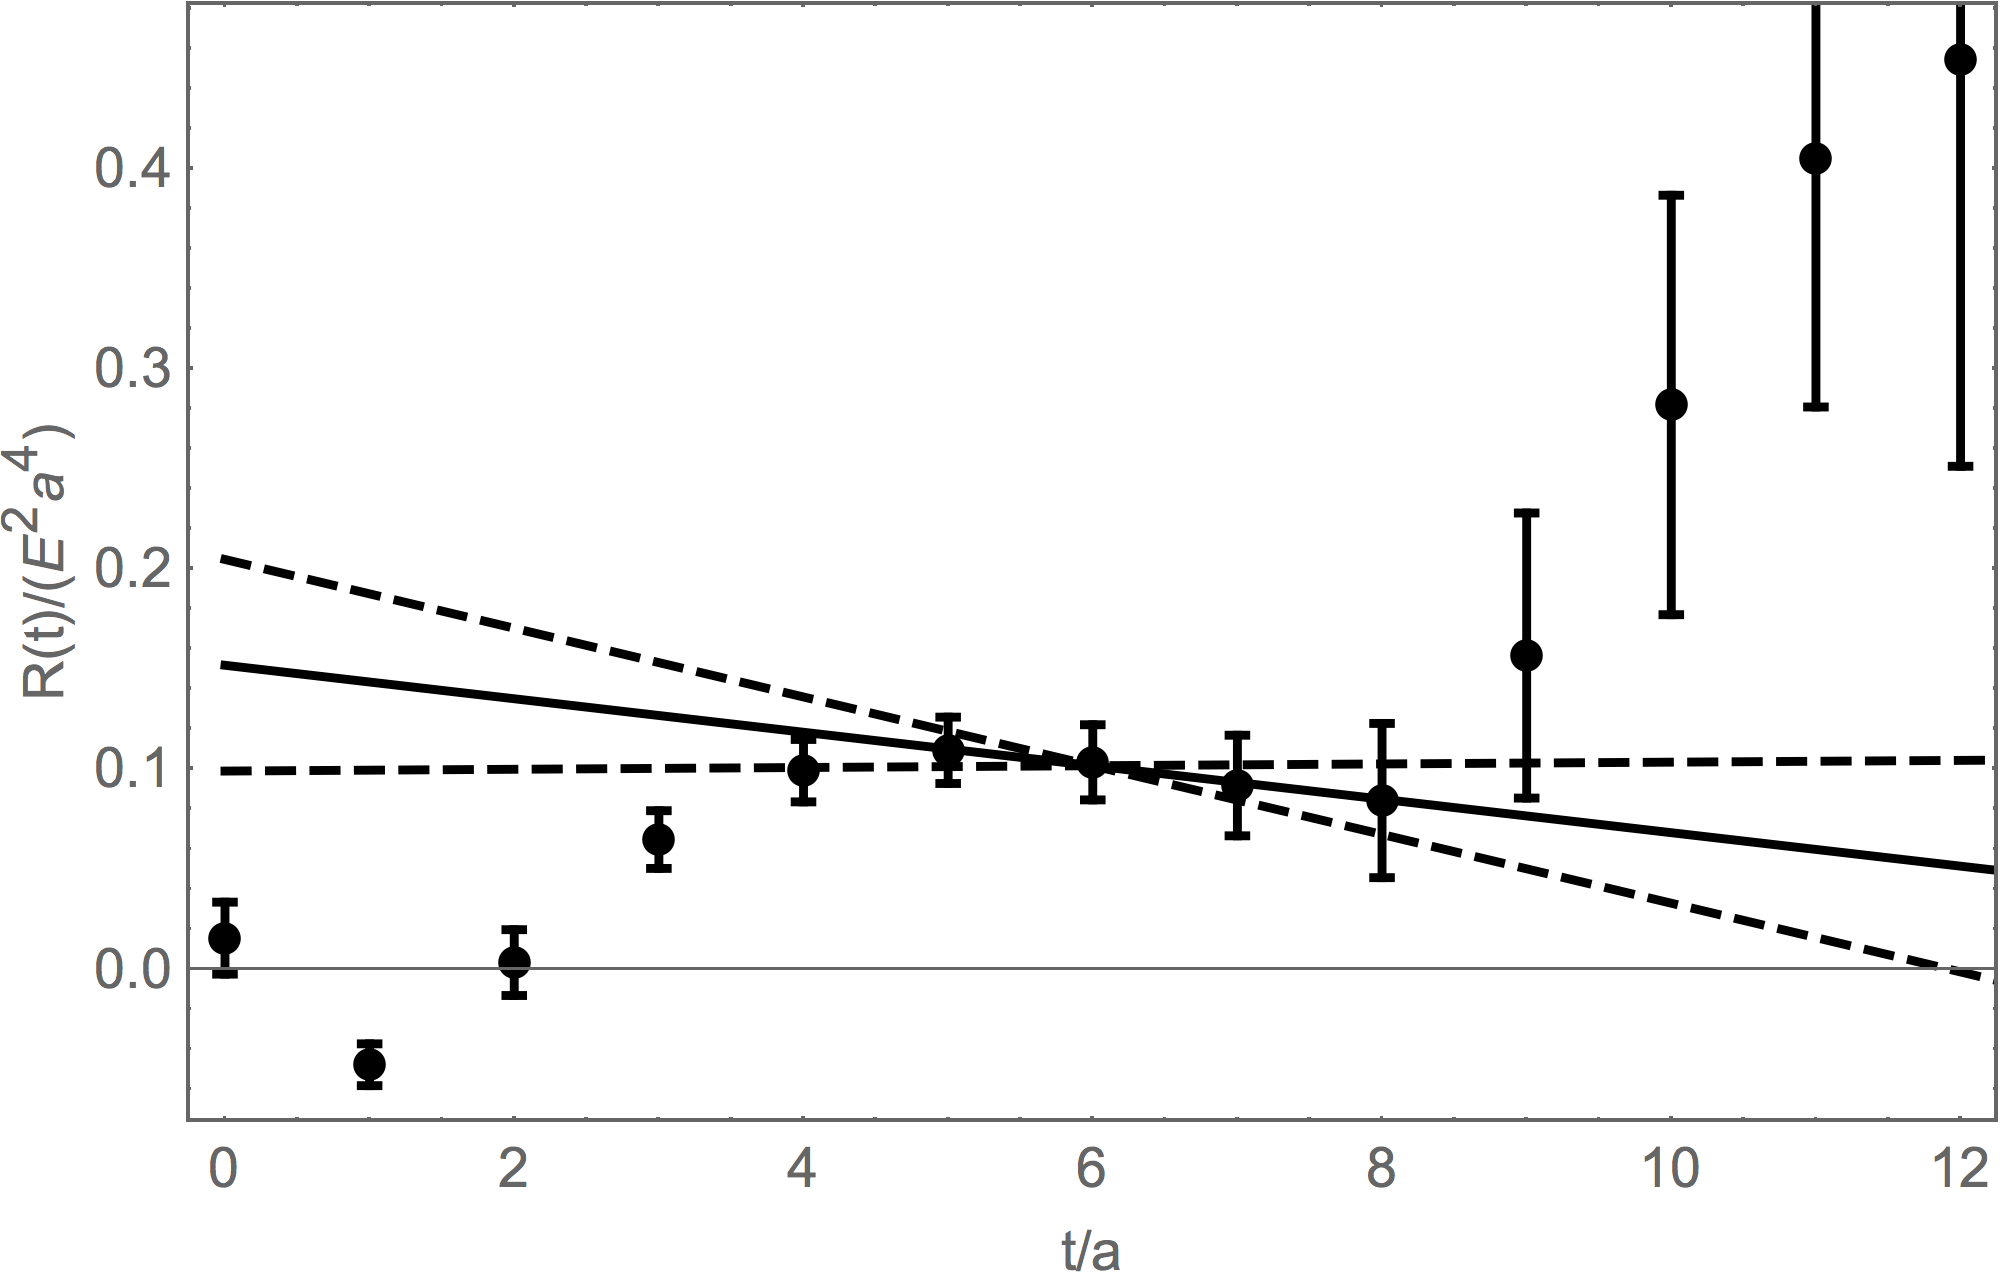
\includegraphics[width=.33\linewidth]{figures/shshLineCS.png}
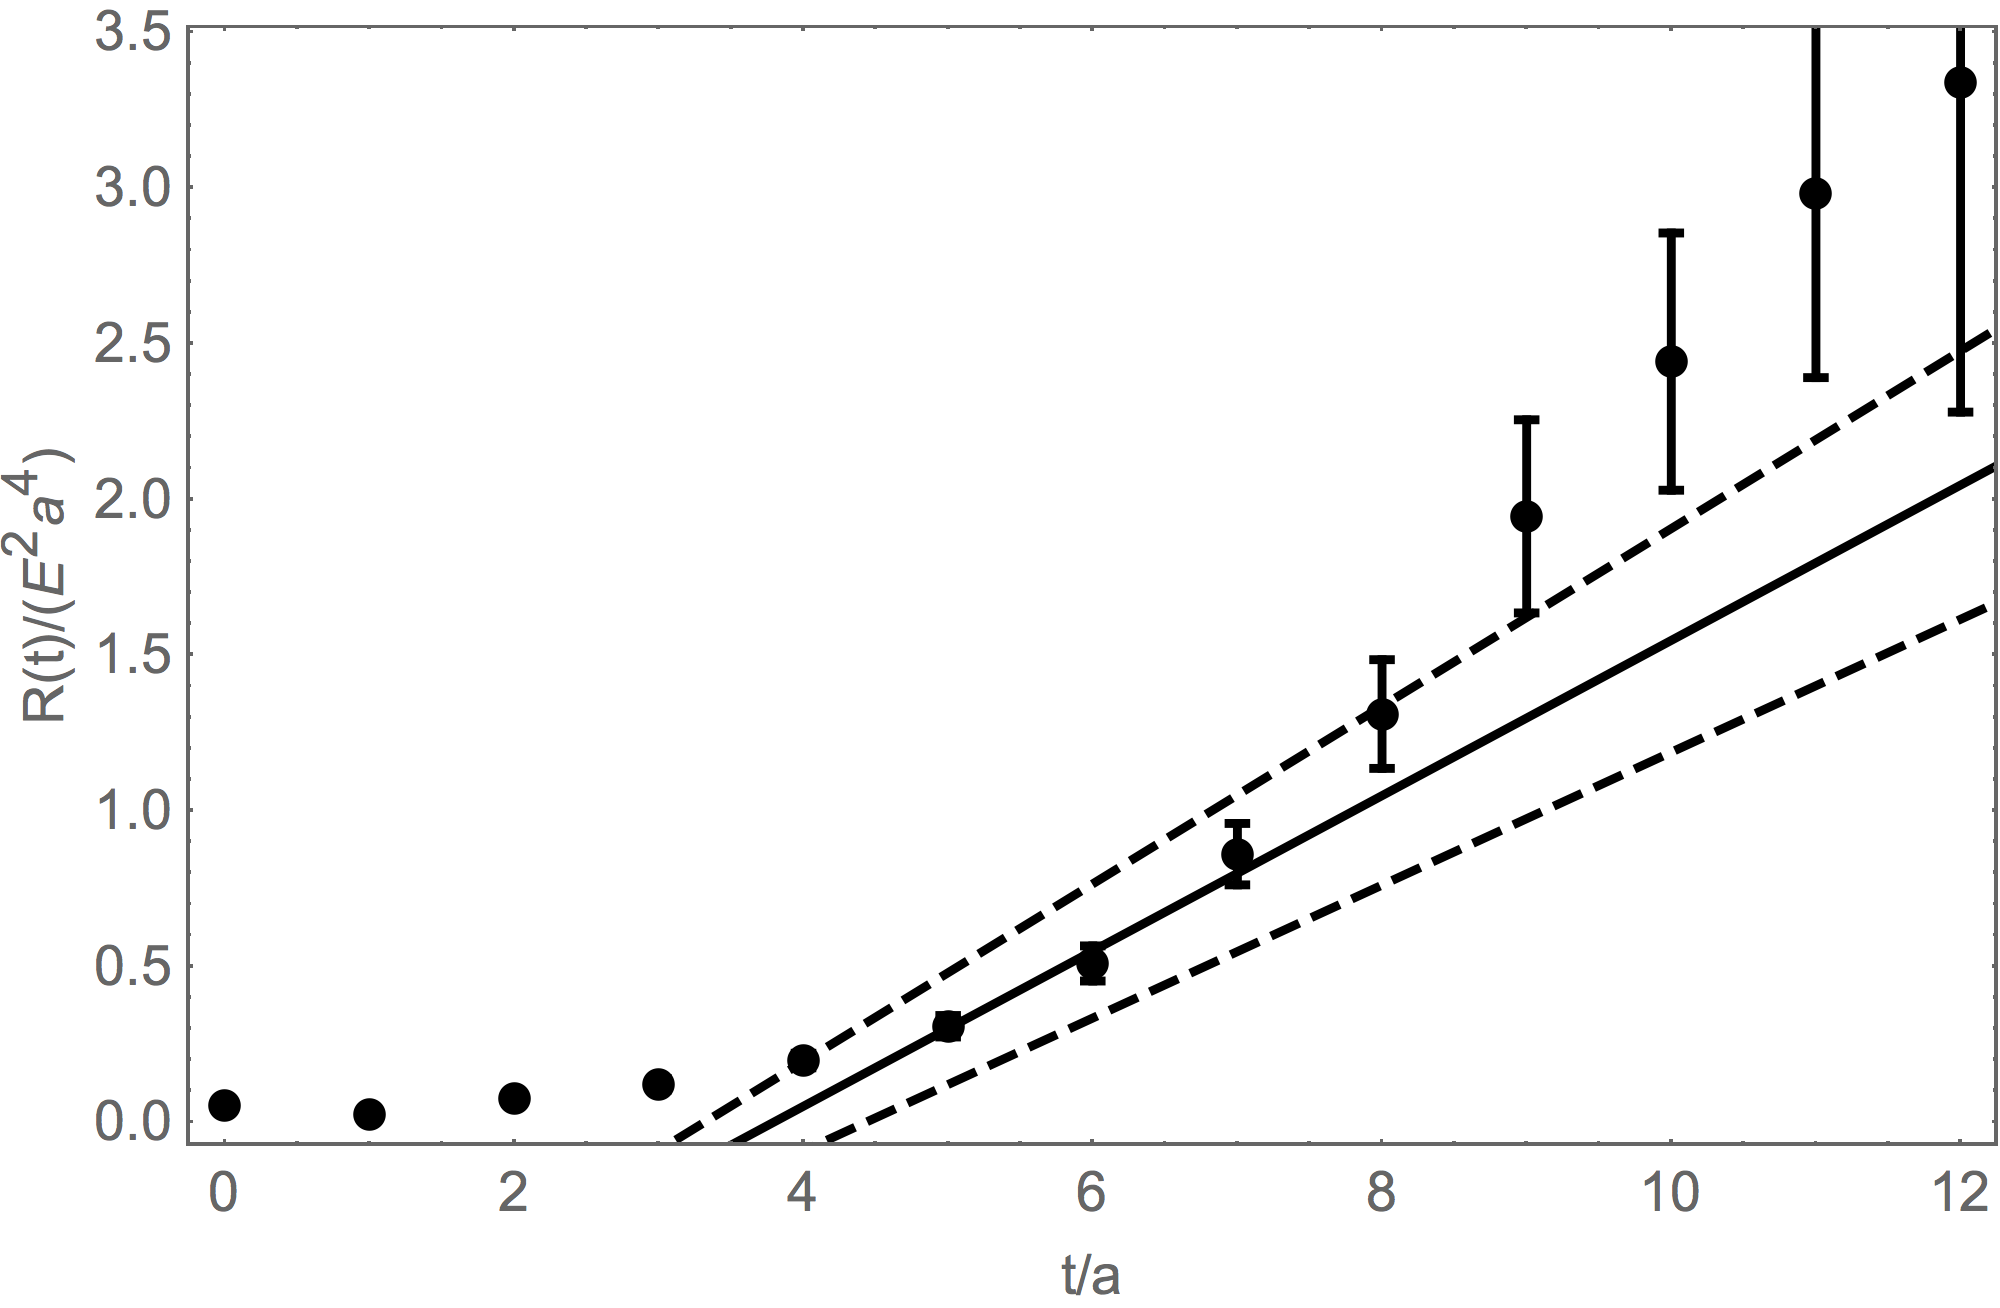
\includegraphics[width=.33\linewidth]{figures/from0LineCS.png}
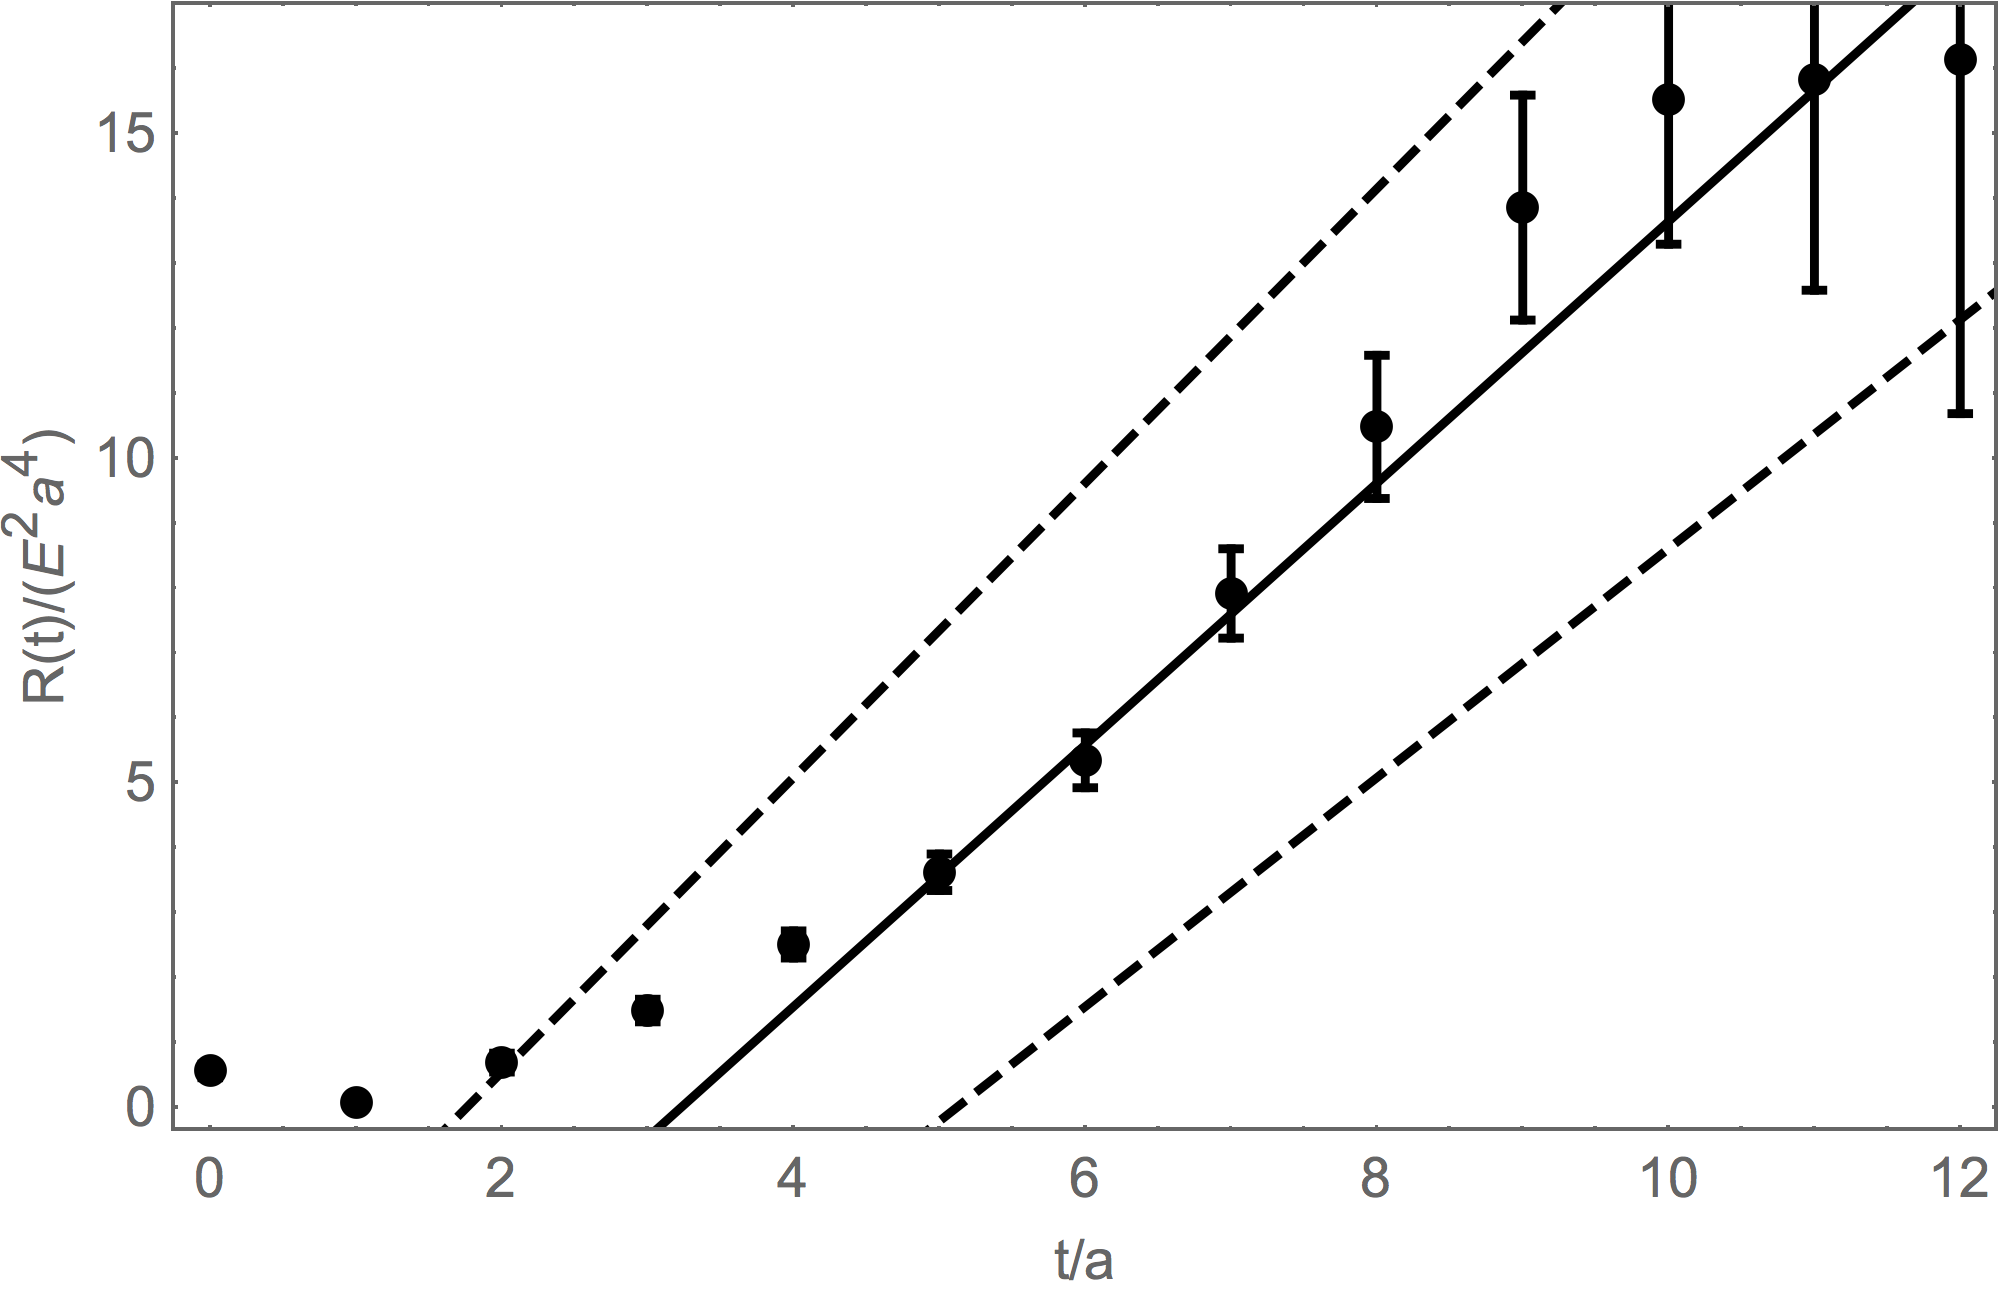
\includegraphics[width=.325\linewidth]{figures/shortLineCS.png}\\
\caption{Correlator ratio $R_2(t)$ and linear fits for the connected diagrams a), b), f), shown in Fig.~\ref{fig:diagrams}, in units of $E^2a^4$. In these plots, the neutron source was placed at the fixed location $t=0$, and the background field, c.f.~\ref{gauge}, was varied with $t_0=6a$, $t_0=0$, $t_0=-10a$ (from left to right). The dashed lines delimit the linear fit uncertainty in the slope.}
\label{fig: alphaconnected}
\end{figure}
%%%%%%%%%%%%%%%%%%%%%%%%%%%%%

%%%%%%%%%Electric Polarizability Results%%%%%
%%%%%%%%%%Multi point Polarizability 10^-4 fm^3%%%%%%
\begin{table}[H]
\begin{center}
    \begin{tabular}{|l|l|l|l|}
    \hline
     Fit range [$t/a$] 					& 5 to 7 		&  4 to 8 		&  3 to 9 \\ \hline
     $\alpha_E$ [$10^{-4}$ $\text{fm}^3$]  	&  0.48(29)      	&  0.57(22)     	& 0.74(16)       \\
								& 0.57(30)		&  0.59(22)	& 0.71(17)		\\ \hline 
     $\alpha_E-\alpha_{FW}$ [$10^{-4}$ $\text{fm}^3$]  	& 0.71(29)   	& 0.79(22)   	&  0.96(16) \\ 
     											& 0.80(30)		& 0.81(22)		& 0.93(17) \\ \hline
    \end{tabular}
\end{center}
\caption{Static electric polarizability  $\alpha_E$ and reduced by the Foldy-Wouthuysen contribution $\alpha_E-\alpha_{FW}$ from the extremal slopes (connected diagrams, $\chi^2$ fits) of the three fitting ranges in units of $10^{-4}$ $\text{fm}^3$. \todo{results from reduced statistics are given in the lower lines}}
\label{tab:ConnectedPolarizabilities}
\end{table}




